% =============================================================================
%  STA6938 Time Series -- Final Project Presentation (15 minutes)
%  Monthly Atmospheric CO2 at Mauna Loa, 1958--2026
%  Compile: pdflatex slides   (speaker notes: pdflatex notes)
% =============================================================================
\documentclass[aspectratio=169,11pt,xcolor=table]{beamer}

\ifdefined\shownotes
  \setbeameroption{show only notes}
\fi

% ---- Theme -------------------------------------------------------------------
\usetheme[progressbar=frametitle, numbering=fraction, sectionpage=none, block=fill]{metropolis}
\usepackage{appendixnumberbeamer}

% ---- Typography: Palatino, matching the report and figures ------------------
\usepackage[T1]{fontenc}
\usepackage[utf8]{inputenc}
\usepackage[sc]{mathpazo}
\usefonttheme{serif}
\usepackage{microtype}
\usepackage{amsmath, amssymb, booktabs, graphicx, tabularx, array}
\urlstyle{same}
\graphicspath{{figures/slide/}{../figures/slide/}{figures/}{../figures/}}

% ---- Colours (Okabe-Ito, as in the figures) ----------------------------------
\definecolor{navy}{HTML}{0B2E4F}
\definecolor{oiblue}{HTML}{0072B2}
\definecolor{oiverm}{HTML}{D55E00}
\definecolor{oigreen}{HTML}{009E73}
\definecolor{paper}{HTML}{FFFFFF}
\definecolor{softgrey}{HTML}{F2F4F7}
\hypersetup{colorlinks=true, urlcolor=oiblue, linkcolor=., pdfauthor={Pascal Antwi}, pdftitle={Modeling and Forecasting Monthly Atmospheric CO2 at Mauna Loa}}
\setbeamercolor{normal text}{fg=black!88, bg=paper}
\setbeamercolor{frametitle}{fg=white, bg=navy}
\setbeamercolor{palette primary}{fg=white, bg=navy}
\setbeamercolor{progress bar}{fg=oiblue, bg=navy!25}
\setbeamercolor{title separator}{fg=oiblue}
\setbeamercolor{alerted text}{fg=oiverm}
\setbeamercolor{example text}{fg=oigreen}
\setbeamercolor{block title}{fg=white, bg=oiblue}
\setbeamercolor{block body}{fg=black!88, bg=softgrey}
\setbeamercolor{block title alerted}{fg=white, bg=oiverm}
\setbeamercolor{block body alerted}{fg=black!88, bg=oiverm!8}
\setbeamercolor{block title example}{fg=white, bg=oigreen}
\setbeamercolor{block body example}{fg=black!88, bg=oigreen!8}
\setbeamerfont{frametitle}{size=\large, series=\bfseries}
\setbeamerfont{block title}{series=\bfseries}
\setbeamertemplate{itemize item}{\color{oiblue}\small$\blacktriangleright$}
\setbeamertemplate{itemize subitem}{\color{oiblue}\scriptsize$\bullet$}
\setlength{\leftmargini}{1.1em}

% ---- Helpers -------------------------------------------------------------------
\newcommand{\co}{CO$_2$}
\newcommand{\ppm}{\,ppm}
\newcommand{\keyfig}[2]{\begin{center}{\Huge\bfseries\color{oiblue}#1}\\[1pt]{\small #2}\end{center}}
\newcommand{\takeaway}[1]{\vfill\begin{beamercolorbox}[wd=\textwidth,sep=5pt,rounded=false]{block body}\small\textbf{\color{oiblue}Takeaway:} #1\end{beamercolorbox}}
\newcolumntype{R}{>{\raggedleft\arraybackslash}X}

% ---- Title -----------------------------------------------------------------------
\title{Modeling and Forecasting Monthly Atmospheric \co\ at Mauna Loa, 1958--2026}
\subtitle{A Seasonal ARIMA Analysis}
\author{Pascal Antwi}
\institute{STA6938 Time Series \quad$\cdot$\quad Final Project}
\date{December 3, 2026}

\begin{document}

% =============================================================================
\maketitle
\note{[0:00 -- 0:20] Good morning. My name is Pascal Antwi. My project is titled Modeling and Forecasting Monthly Atmospheric CO2 at Mauna Loa, 1958 to 2026. I will show how the series was made stationary, how a seasonal ARIMA model was identified, tested and validated, and what it forecasts up to 2030.}

% =============================================================================
\begin{frame}{Roadmap}
\begin{columns}[T]
\column{0.5\textwidth}
\begin{enumerate}
  \item Background, motivation and data
  \item Trend, seasonality and stationarity
  \item Model identification and selection
  \item Estimation, tests and confidence intervals
  \item Model adequacy and remedial measures
  \item Forecast evaluation and forecasts to 2030
\end{enumerate}
\column{0.45\textwidth}
\begin{block}{Research questions}
\begin{itemize}
  \item How fast is \co\ rising?
  \item Is the rise accelerating?
  \item What levels should we expect by 2030?
\end{itemize}
\end{block}
\end{columns}
\note{[0:20 -- 0:50] The presentation follows the Box--Jenkins approach. I begin with the background and the data, then examine trend, seasonality and stationarity. Next I identify and select a model, report the estimates with hypothesis tests and confidence intervals, check model adequacy and apply remedial measures, and finally evaluate and present the forecasts. Three questions guide the analysis: how fast CO2 is rising, whether the rise is accelerating, and what levels should be expected by 2030.}
\end{frame}

% =============================================================================
\begin{frame}{Background and motivation}
\begin{columns}[T]
\column{0.48\textwidth}
\begin{block}{Rationale}
\small
\begin{itemize}
  \item \co\ is the principal driver of anthropogenic climate change.
  \item Climate targets depend on \emph{how fast} \co\ rises and \emph{when} it crosses thresholds.
  \item Rigorous characterization and forecasting are of direct scientific and policy relevance.
  \item Methodologically rich: stochastic trend, seasonal cycle and serial dependence.
\end{itemize}
\end{block}
\column{0.48\textwidth}
\begin{alertblock}{The question}
\small
\co\ is rising; the question is \textbf{how fast}, \textbf{whether it is accelerating}, and \textbf{what to expect next}, with proper uncertainty.
\end{alertblock}
\begin{exampleblock}{Objectives}
\small
\begin{enumerate}\setlength{\itemsep}{0pt}
  \item Characterize the trend and seasonality.
  \item Build and validate an adequate model.
  \item Test whether growth is accelerating.
  \item Forecast to 2030 with prediction intervals.
\end{enumerate}
\end{exampleblock}
\end{columns}
\note{[0:50 -- 2:00] Carbon dioxide is the principal driver of anthropogenic climate change, and international climate targets are framed around how fast its concentration rises and when it crosses particular thresholds, such as 440 parts per million. A rigorous statistical characterization and forecast of the Mauna Loa record is therefore of direct scientific and policy relevance. The series is also well suited to time series methodology, because it combines a stochastic trend, a pronounced seasonal cycle and short-term serial dependence. The question is not whether CO2 is rising, which is well established, but how fast it is rising, whether the rise is accelerating, and what levels to expect, each with proper statistical uncertainty. The four objectives on the right follow directly from that question.}
\end{frame}

% =============================================================================
\begin{frame}{The data: Mauna Loa monthly \co}
\begin{columns}[T]
\column{0.52\textwidth}
\begin{itemize}
  \item Mauna Loa Observatory, Hawaii: the longest continuous direct \co\ record, started by C.~D.~Keeling in 1958.
  \item \textbf{Source:} NOAA Global Monitoring Laboratory [2],\\ {\small\url{https://gml.noaa.gov/ccgg/trends/data.html}}
  \item \textbf{Variable:} monthly mean mole fraction, in parts per million (ppm).
  \item Real, public and never analyzed by me before; a large sample for time series modeling.
\end{itemize}
\column{0.44\textwidth}
\begin{block}{The series at a glance}
\begin{tabular*}{\linewidth}{@{}l@{\extracolsep{\fill}}r@{}}
Months, $n$ & 822\\
Period & 1958--2026\\
Missing values & none\\
First value & 315.71\ppm\\
Last value & 427.55\ppm\\
Increase & \alert{+111.8\ppm}\\
Relative increase & \alert{35\%}\\
\end{tabular*}
\end{block}
\end{columns}
\note{[2:00 -- 2:40] The data are the monthly mean CO2 concentrations published by the NOAA Global Monitoring Laboratory, which are freely available online. The record contains 822 consecutive months, from March 1958 to August 2026, with no missing values, which is a large sample for time series modeling. Over this period the concentration rose from 315.7 to 427.6 parts per million, an increase of about 112 parts per million, or 35 percent.}
\end{frame}

% =============================================================================
\begin{frame}{Step 1: the time plot}
\begin{center}
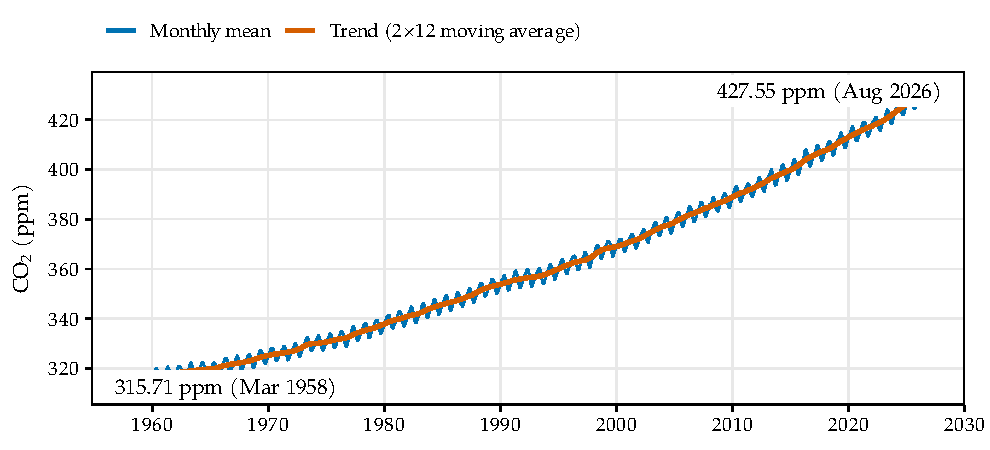
\includegraphics[width=0.9\textwidth]{fig01_co2_series.pdf}
\end{center}
\vspace{-6pt}
\takeaway{An \alert{upward trend} and a regular \alert{12-month cycle}: the mean depends on $t$, so the series is non-stationary.}
\note{[2:40 -- 3:20] Following standard practice, the first step was the time plot. Two features are immediately visible. First, there is a persistent upward trend, so the mean of the series depends on time. Second, there is a regular twelve-month seasonal cycle with almost the same shape every year. The series is therefore clearly non-stationary, and both the trend and the seasonal component must be addressed before an ARMA-type model can be fitted.}
\end{frame}

% =============================================================================
\begin{frame}{Decomposition: trend plus a stable seasonal cycle}
\begin{columns}[c]
\column{0.5\textwidth}
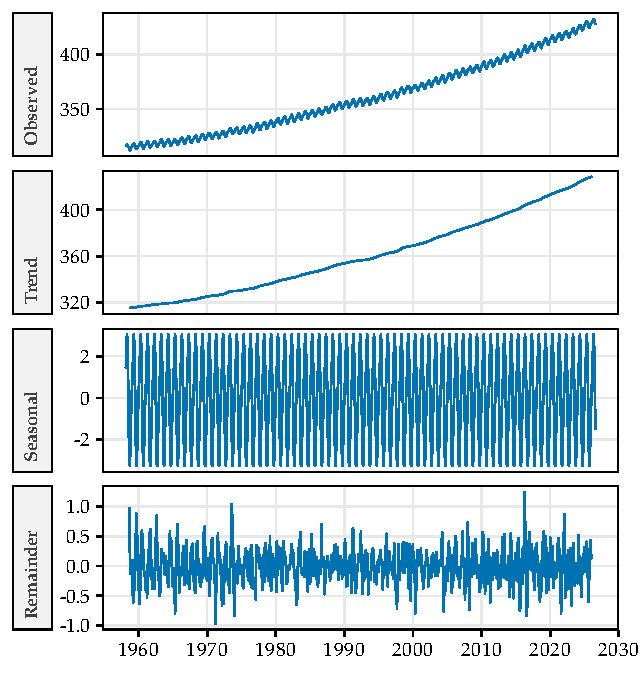
\includegraphics[width=\linewidth]{fig02_classical_decomposition.pdf}
\column{0.48\textwidth}
\small
\begin{itemize}
  \item Additive, $2\times12$ moving-average filter.
  \item Trend: \alert{96.6\%} of the variance.
  \item Peak in \textbf{May} ($+3.04$\ppm), trough in \textbf{October} ($-3.25$\ppm); amplitude \textbf{6.29\ppm}.
  \item Amplitude 6.0\ppm\ (1960s) vs 7.0\ppm\ (2010s), while the level rose 35\%.
\end{itemize}
\begin{exampleblock}{Decision}
Swings do not grow with the level $\Rightarrow$ \textbf{additive model, no transformation}.
\end{exampleblock}
\end{columns}
\note{[3:20 -- 4:15] A classical additive decomposition with a two-by-twelve moving-average filter separates these components. The trend accounts for about 97 percent of the variance. The seasonal component peaks in May and reaches its minimum in October, with an amplitude of about 6.3 parts per million, reflecting the uptake of carbon by Northern Hemisphere vegetation during the growing season. An important modeling decision follows from this panel: the seasonal amplitude rose only from about 6.0 to 7.0 parts per million while the level rose by 35 percent. The seasonal swings do not grow in proportion to the level, so an additive model is appropriate and no log or Box--Cox transformation is required.}
\end{frame}

% =============================================================================
\begin{frame}{The growth rate is accelerating}
\begin{center}
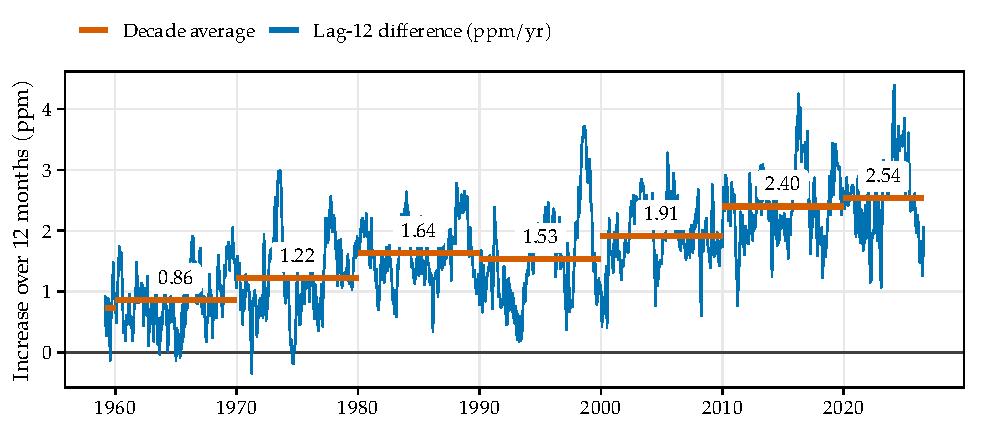
\includegraphics[width=0.9\textwidth]{fig06_annual_growth_lag12_difference.pdf}
\end{center}
\vspace{-6pt}
\takeaway{Growth tripled: \alert{0.86\ppm/yr} (1960s) $\rightarrow$ \alert{2.54\ppm/yr} (2020s). Record jumps in El Niño years (2016, 2024).}
\note{[4:15 -- 5:00] This figure shows the twelve-month change, which is the annual growth in concentration. The decade averages rise from 0.86 parts per million per year in the 1960s to 2.54 in the 2020s, so the growth rate has roughly tripled. In other words, CO2 is not only increasing but increasing faster. The largest twelve-month increases occurred in 2016 and 2024, both strong El Nino years, which will matter later when we examine the residuals and the forecasts.}
\end{frame}

% =============================================================================
\begin{frame}{Achieving stationarity}
\begin{columns}[c]
\column{0.43\textwidth}
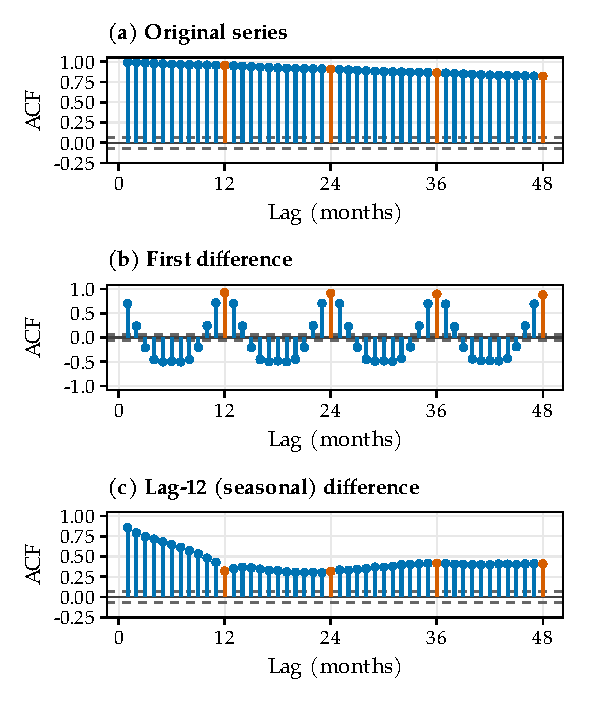
\includegraphics[width=\linewidth]{fig05_acf_original_and_differences.pdf}
\column{0.55\textwidth}
\small
\begin{itemize}
  \item $X_t$: ACF outside the 95\% CI ($\pm0.068$) at every lag; decays very slowly.
  \item $\nabla X_t$: ACF $\approx 0.9$ at lags 12, 24, 36 $\Rightarrow$ seasonal difference.
  \item $\nabla_{12}X_t$: slow decay $\Rightarrow$ regular difference.
\end{itemize}
\vspace{2pt}
\footnotesize
\begin{tabular}{@{}llrc@{}}
\toprule
\multicolumn{4}{@{}l}{\textbf{Augmented Dickey--Fuller}, $H_0$: unit root}\\
\midrule
Series & Type & $\tau$ & Decision\\
\midrule
Seas.\ adj.\ $X_t$ & mean & 3.57 to 4.85 & keep $H_0$\\
Seas.\ adj.\ $X_t$ & trend & $-0.88$ to $-0.62$ & keep $H_0$\\
$\nabla\nabla_{12}X_t$ & mean & $-37.9$ to $-22.1$ & \alert{reject}\\
\bottomrule
\end{tabular}
\vspace{4pt}

\small $\Rightarrow\; W_t = (1-B)(1-B^{12})X_t$ is \textbf{stationary}.
\end{columns}
\note{[5:00 -- 6:00] The sample ACF confirms the non-stationarity. The shaded band is the 95 percent confidence interval, plus or minus 1.96 over root n, about 0.068. For the original series every autocorrelation lies far outside this band, and it decays extremely slowly from 0.996. After a first difference, the autocorrelations at the seasonal lags 12, 24 and 36 remain around 0.9, which shows that a seasonal difference is also needed. After the seasonal difference alone, the ACF still decays slowly, so a regular difference is needed as well. The Augmented Dickey--Fuller test agrees: for the seasonally adjusted series the unit-root hypothesis cannot be rejected, whereas after both differences it is rejected decisively. The stationary series used for modeling is therefore W sub t, the regular and seasonal difference of the data.}
\end{frame}

% =============================================================================
\begin{frame}{Estimation versus differencing}
\begin{columns}[c]
\column{0.58\textwidth}
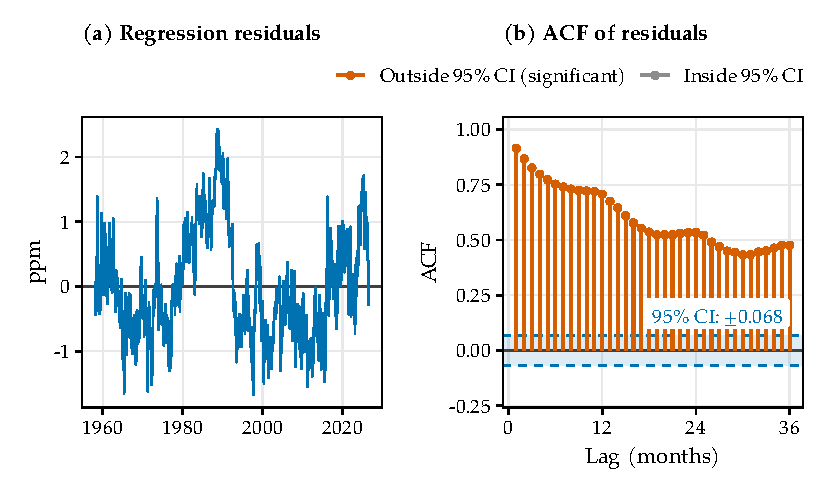
\includegraphics[width=\linewidth]{fig09_regression_residuals.pdf}
\column{0.4\textwidth}
\small
Quadratic trend + 11 monthly dummies:
\begin{itemize}
  \item Fit: $R^2 = 0.9994$.
  \item Residual ACF(1) $=0.915$; $Q(12)=5991$.
  \item Durbin--Watson $D = \alert{0.17}$ ($\ll 2$).
  \item ARMA errors: AR root 1.02.
\end{itemize}
\begin{alertblock}{Conclusion}
Deterministic trend fails: \textbf{difference instead}.
\end{alertblock}
\end{columns}
\note{[6:00 -- 6:45] As an alternative to differencing, I estimated the trend and seasonality deterministically, by regressing the series on a quadratic trend and eleven monthly dummy variables. The fit appears excellent, with an R-squared of 0.9994. However, the residuals are far from white noise: their lag-one autocorrelation is 0.915 and the Durbin--Watson statistic is 0.17, far below the value of 2 expected under independence. Even when the errors are modeled as an ARMA process, the autoregressive root is essentially one. The deterministic approach is therefore inadequate, and differencing is the appropriate treatment.}
\end{frame}

% =============================================================================
\begin{frame}{Identification from the ACF and PACF of $W_t$}
\begin{columns}[c]
\column{0.48\textwidth}
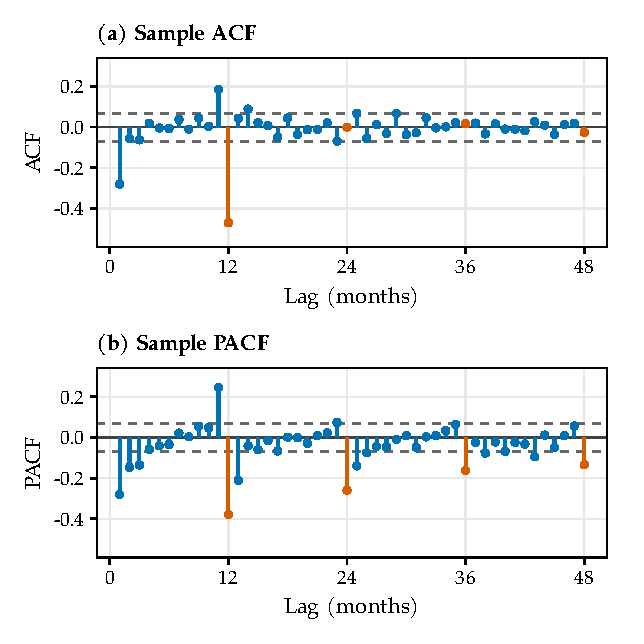
\includegraphics[width=\linewidth]{fig08_acf_pacf_differenced.pdf}
\column{0.5\textwidth}
\small
\begin{itemize}
  \item $Q(12)=283.3$, $p<0.001$: $W_t$ is not white noise.
  \item 95\% CI: $\pm1.96/\sqrt{809}=\pm0.069$.
  \item \textbf{ACF cuts off}: outside the CI only at lags 1 ($-0.28$), 11 and 12 ($-0.47$).
  \item \textbf{PACF tails off}: outside the CI at lags 1--3 and 12, 24, 36.
  \item $\Rightarrow$ MA(1) $\times$ seasonal MA(1).
\end{itemize}
\begin{block}{ARIMA$(0,1,1)\times(0,1,1)_{12}$}
\vspace{-6pt}
\[(1-B)(1-B^{12})X_t=(1-\theta_1B)(1-\Theta_1B^{12})Z_t\]
\vspace{-10pt}
\end{block}
\end{columns}
\note{[6:45 -- 7:45] The Ljung--Box test shows that the differenced series is not white noise, so its dependence must be modeled. Significance is judged against the shaded 95 percent confidence band of plus or minus 0.069; spikes outside it are shown in orange. The sample ACF lies clearly outside the band only at lags 1 and 12, together with the satellite lag 11, and then cuts off. The sample PACF lies outside the band at lags 1 to 3 and again at the seasonal lags 12, 24 and 36, decaying gradually, so it tails off. An ACF that cuts off together with a PACF that tails off is the signature of moving-average behavior, here at both the non-seasonal and the seasonal level. This identifies the multiplicative seasonal ARIMA model with one regular and one seasonal moving-average term, shown in the box.}
\end{frame}

% =============================================================================
\begin{frame}{Model selection: AIC and SBC}
\centering\small
\begin{tabular}{@{}lcrrrc@{}}
\toprule
Model & Parameters & AIC & SBC & $\Delta$SBC & Ljung--Box $Q(24)$ $p$\\
\midrule
\rowcolor{oiblue!10}\textbf{ARIMA$(0,1,1)\times(0,1,1)_{12}$} & \textbf{2} & 451.30 & \textbf{465.39} & \textbf{0.00} & 0.532\\
ARIMA$(1,1,1)\times(0,1,1)_{12}$ & 3 & \textbf{447.58} & 466.37 & 0.98 & 0.769\\
ARIMA$(0,1,2)\times(0,1,1)_{12}$ & 3 & 448.59 & 467.38 & 1.99 & 0.723\\
ARIMA$(0,1,1)\times(1,1,1)_{12}$ & 3 & 453.30 & 472.08 & 6.69 & 0.472\\
ARIMA$(2,1,0)\times(0,1,1)_{12}$ & 3 & 460.64 & 479.42 & 14.03 & 0.213\\
ARIMA$(1,1,0)\times(0,1,1)_{12}$ & 2 & 472.83 & 486.92 & 21.53 & 0.038\\
ARIMA$(0,1,1)\times(1,1,0)_{12}$ & 2 & 669.34 & 683.43 & 218.04 & $<0.001$\\
\bottomrule
\end{tabular}
\vspace{10pt}
\begin{itemize}
  \item Nine candidates fitted by maximum likelihood; \textbf{SBC} preferred in this large sample.
  \item Pure AR and seasonal-AR alternatives fit clearly worse.
\end{itemize}
\note{[7:45 -- 8:30] To confirm the identification, nine candidate models were estimated by maximum likelihood, including models with additional autoregressive, moving-average and seasonal autoregressive terms. The identified two-parameter model has the lowest Schwarz Bayesian criterion. One richer model has a slightly lower AIC, but SBC penalizes additional parameters more heavily, which is appropriate in a large sample. Pure autoregressive and seasonal autoregressive alternatives fit clearly worse, consistent with the identification on the previous slide.}
\end{frame}

% =============================================================================
\begin{frame}{Four model families compared}
\centering\footnotesize
\begin{tabular}{@{}llccc@{}}
\toprule
Family & Best model (by SBC) & ACF lag 12 & $Q(12)$ $p$ & White noise?\\
\midrule
ARMA & ARMA(3,2) for $W_t$ & $-0.409$ & $<0.001$ & \alert{No}\\
ARIMA & ARIMA(4,1,4) with drift & $0.180$ & $<0.001$ & \alert{No}\\
Regression + ARMA errors & ARMA(2,1) errors & $0.138$ & $<0.001$ & \alert{No}\\
\rowcolor{oiblue!10}\textbf{Seasonal ARIMA} & \textbf{ARIMA$(0,1,1)\times(0,1,1)_{12}$} & $\mathbf{-0.005}$ & \textbf{0.464} & \textcolor{oigreen}{\textbf{Yes}}\\
\bottomrule
\end{tabular}
\vspace{10pt}
\begin{itemize}
  \item Non-seasonal ARIMA mimics the seasonal difference with AR roots \emph{on} the unit circle (periods 6 and 12).
  \item Only the seasonal ARIMA captures the seasonal structure, with just \textbf{two parameters}.
\end{itemize}
\note{[8:30 -- 9:30] I also compared four model families: ARMA, ARIMA, regression with autocorrelated errors, and seasonal ARIMA, choosing the best order within each family by SBC. Only the seasonal ARIMA leaves white-noise residuals; the other three retain significant autocorrelation at lag 12. The best non-seasonal ARIMA even places its autoregressive roots exactly on the unit circle, at periods of 6 and 12 months, in effect imitating a seasonal difference. The seasonal ARIMA captures the full structure with only two parameters.}
\end{frame}

% =============================================================================
\begin{frame}{Estimates, hypothesis tests and confidence intervals}
\centering\small
\begin{tabular}{@{}llrrrrc@{}}
\toprule
Method & Parameter & Estimate & SE & $z$ & $p$ & 95\% CI\\
\midrule
Maximum likelihood & $\theta_1$ & 0.3885 & 0.0367 & 10.59 & $<0.001$ & [0.317, 0.460]\\
 & $\Theta_1$ & 0.8700 & 0.0170 & 51.28 & $<0.001$ & [0.837, 0.903]\\
\midrule
Conditional least squares & $\theta_1$ & 0.4172 & 0.0360 & 11.60 & $<0.001$ & [0.347, 0.488]\\
 & $\Theta_1$ & 0.8116 & 0.0194 & 41.84 & $<0.001$ & [0.774, 0.850]\\
\bottomrule
\end{tabular}
\vspace{6pt}
\begin{columns}[T]
\column{0.48\textwidth}
\begin{block}{Inference}
\small Both parameters highly significant; ML and CLS agree. $\hat\sigma_Z = 0.318$\ppm.\\
Invertible: roots $2.57$ and $1.012 > 1$.
\end{block}
\column{0.48\textwidth}
\begin{exampleblock}{Interpretation}
\small $\hat\theta_1$: 39\% of a monthly shock reverses next month.\\
$\hat\Theta_1 = 0.87$: very stable seasonal pattern; CI excludes 1.
\end{exampleblock}
\end{columns}
\note{[9:30 -- 10:30] This slide reports the hypothesis tests and confidence intervals. The non-seasonal coefficient theta is 0.389 and the seasonal coefficient capital theta is 0.870. Both are highly significant, with z-statistics of 10.6 and 51.3, and their 95 percent confidence intervals exclude zero. Conditional least squares gives very similar values, so the conclusions do not depend on the estimation method. All roots lie outside the unit circle, so the model is invertible and suitable for forecasting. In interpretation, about 39 percent of each monthly shock is reversed the following month, and the large seasonal coefficient indicates a very stable seasonal pattern. Because its confidence interval excludes one, seasonal differencing is justified.}
\end{frame}

% =============================================================================
\begin{frame}{Model adequacy: residual diagnostics}
\begin{columns}[c]
\column{0.56\textwidth}
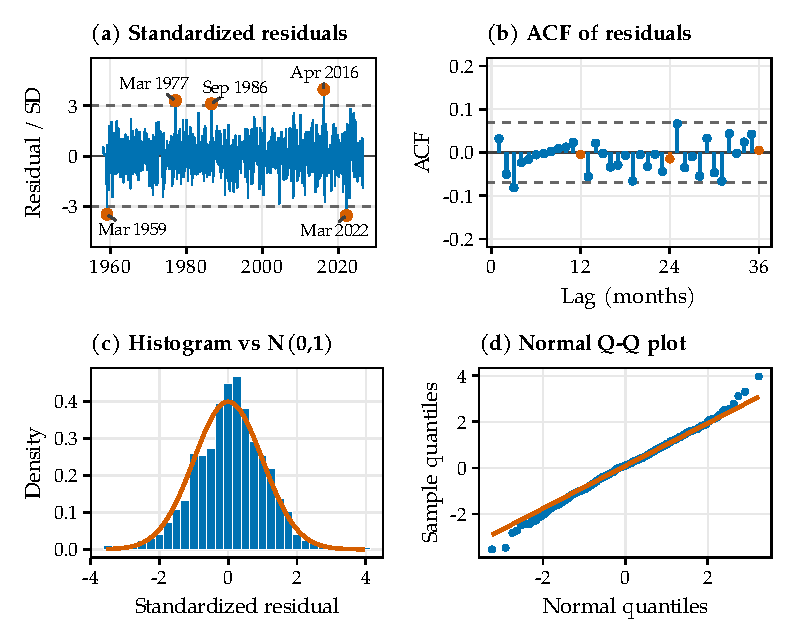
\includegraphics[width=\linewidth]{fig10_final_model_residual_diagnostics.pdf}
\column{0.42\textwidth}
\footnotesize
\begin{tabular}{@{}lrr@{}}
\toprule
Test & Statistic & $p$\\
\midrule
Ljung--Box $Q(6)$ & 9.05 & 0.060\\
Ljung--Box $Q(12)$ & 9.74 & 0.464\\
Ljung--Box $Q(18)$ & 14.43 & 0.567\\
Ljung--Box $Q(24)$ & 20.83 & 0.532\\
$Q(12)$, squared resid. & 12.40 & 0.414\\
Shapiro--Wilk & 0.996 & 0.048\\
\bottomrule
\end{tabular}
\vspace{4pt}
\small
\begin{itemize}
  \item Independence \textcolor{oigreen}{\checkmark} \; Constant variance \textcolor{oigreen}{\checkmark}
  \item Normality \alert{marginal}: 5 months beyond $\pm3$.
\end{itemize}
\end{columns}
\note{[10:30 -- 11:20] Model adequacy was checked on the residuals. In the residual ACF, only lag 3 falls just outside the 95 percent confidence band, which is about what chance alone would produce over 36 lags. The residuals also pass the Ljung--Box test at lags 6, 12, 18 and 24, so they are consistent with white noise, and the Ljung--Box test on the squared residuals shows no change in variance over time. Normality is only marginally rejected by the Shapiro--Wilk test, at a p-value of 0.048. This is driven by five months with standardized residuals beyond plus or minus three, including April 2016, during a strong El Nino.}
\end{frame}

% =============================================================================
\begin{frame}{Remedial measures}
\begin{columns}[T]
\column{0.48\textwidth}
\begin{block}{1. Small lag-3 autocorrelation}
\small
Added an AR(1) term: $\hat\phi_1 = 0.215$ ($p=0.010$).
\begin{itemize}
  \item SBC rises (466.37 vs 465.39).
  \item Hold-out RMSE worse: 1.168 vs 1.110.
  \item Interval coverage only \alert{83\%} vs 97\%.
\end{itemize}
$\Rightarrow$ \textbf{Rejected}: keep the parsimonious model.
\end{block}
\column{0.48\textwidth}
\begin{block}{2. Five outlying months}
\small
Re-estimated with those months set to missing:
\begin{itemize}
  \item $\hat\theta_1 = 0.384$, $\hat\Theta_1 = 0.869$: \textbf{unchanged}.
  \item Normality restored: Shapiro--Wilk $p=0.211$, Anderson--Darling $p=0.101$.
\end{itemize}
$\Rightarrow$ Inference is \textbf{robust}.
\end{block}
\end{columns}
\takeaway{ARIMA$(0,1,1)\times(0,1,1)_{12}$ is adequate; no transformation is needed.}
\note{[11:20 -- 12:10] Two remedial measures were considered. First, a small residual autocorrelation at lag 3 suggested adding an autoregressive term. The extended model has a significant AR coefficient, but its SBC is higher and, out of sample, it forecasts less accurately and its 95 percent intervals cover only 83 percent of outcomes. It was therefore rejected in favor of the parsimonious model. Second, the five outlying months were treated as missing and the model re-estimated. The estimates were essentially unchanged and normality was no longer rejected, so the inference is robust.}
\end{frame}

% =============================================================================
\begin{frame}{Forecast evaluation}
\begin{columns}[c]
\column{0.58\textwidth}
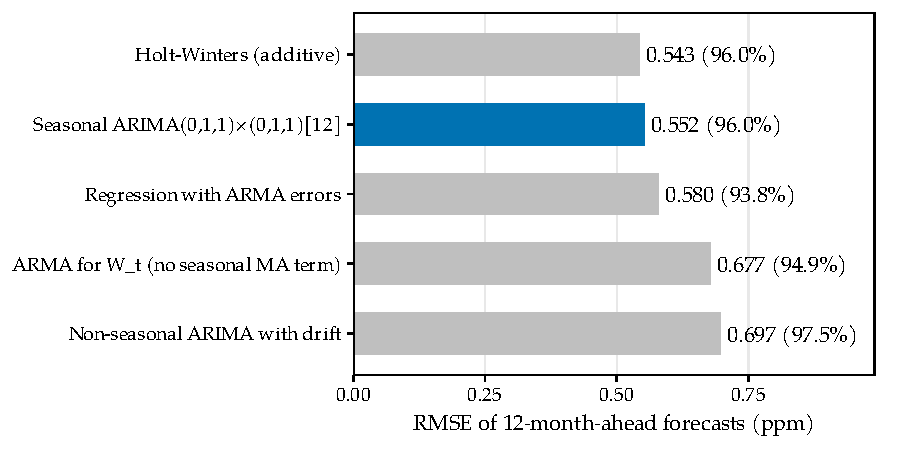
\includegraphics[width=\linewidth]{fig15_rolling_origin_accuracy.pdf}
\column{0.4\textwidth}
\small
\textbf{Rolling origin:} refit each August 2000--2022; forecast 12 months (276 forecasts).
\begin{itemize}
  \item Seasonal ARIMA: RMSE \alert{0.552\ppm}, 95\% coverage \alert{96.0\%}.
  \item Best of the four model families; tied with Holt--Winters smoothing.
\end{itemize}
\textbf{Hold-out} (Sep 2023 -- Aug 2026): RMSE 1.110\ppm, coverage 97.2\%.
\end{columns}
\note{[12:10 -- 13:00] Forecast performance was evaluated with a rolling-origin design: each model was re-estimated every August from 2000 to 2022 and used to forecast the following twelve months, giving 276 out-of-sample forecasts. The seasonal ARIMA achieved an RMSE of about 0.55 parts per million, with 95 percent interval coverage of 96 percent, close to the nominal level. It is the most accurate of the four model families and essentially tied with Holt--Winters exponential smoothing. On the most recent three-year hold-out, its intervals covered 97 percent of the observations.}
\end{frame}

% =============================================================================
\begin{frame}{Forecasts to 2030}
\begin{columns}[c]
\column{0.6\textwidth}
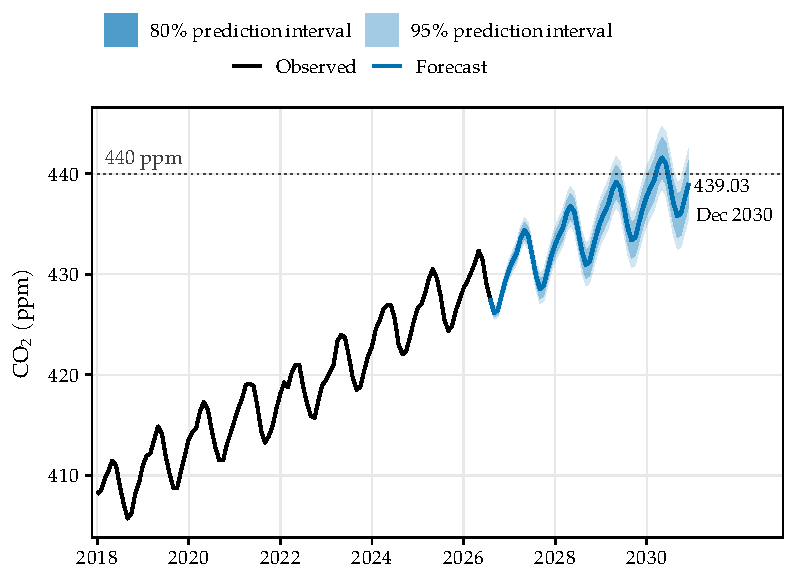
\includegraphics[width=\linewidth]{fig13_forecast_to_2030.pdf}
\column{0.38\textwidth}
\keyfig{April 2030}{\co\ first exceeds \textbf{440\ppm}\\ 440.84\ppm\ [437.78, 443.89]}
\small
\begin{itemize}
  \item Dec 2030: 439.03\ppm\\ 95\% PI [435.59, 442.47]
  \item Growth $\approx$ \textbf{2.4\ppm/yr}
  \item Holt--Winters agrees within 0.13\ppm.
\end{itemize}
\end{columns}
\note{[13:00 -- 13:50] Finally, the model estimated on all 822 months was used to forecast to the end of 2030. Monthly CO2 is forecast to exceed 440 parts per million for the first time in April 2030, with a 95 percent prediction interval of roughly 438 to 444. Concentrations continue to rise by about 2.4 parts per million per year, and the prediction intervals widen with the horizon, reflecting the accumulated uncertainty of a doubly differenced process.}
\end{frame}

% =============================================================================
\begin{frame}{Conclusions}
\small
\begin{enumerate}
  \item \co\ is non-stationary with an \textbf{accelerating trend} and a \textbf{stable 12-month cycle}; regular and seasonal differencing achieve stationarity.
  \item \textbf{ARIMA$(0,1,1)\times(0,1,1)_{12}$} is selected by ACF/PACF identification and SBC; both parameters are highly significant and the model is invertible.
  \item Residuals are white noise with constant variance; inference is robust to five outlying months.
  \item Best of four model families in out-of-sample forecasting (RMSE 0.55\ppm, 96\% coverage).
  \item \co\ rises $\approx$\,2.4\ppm/yr and is forecast to pass \alert{440\ppm\ in April 2030}.
\end{enumerate}
\begin{alertblock}{Limitations and extensions}
\small Univariate model: it cannot anticipate El Niño surges (2016, 2024). Adding climate indices or emissions data is a natural extension.
\end{alertblock}
\note{[13:50 -- 14:50] To conclude, monthly CO2 at Mauna Loa is non-stationary, with an accelerating trend and a stable seasonal cycle, and both a regular and a seasonal difference are required. The seasonal ARIMA model with one regular and one seasonal moving-average term was selected by identification and SBC. Both parameters are highly significant, the model is invertible, and its residuals are white noise. It outperforms the other model families out of sample. The results show that CO2 is rising at about 2.4 parts per million per year and is forecast to pass 440 parts per million in April 2030. The main limitation is that a univariate model cannot anticipate El Nino-driven surges; incorporating climate indices or emissions data is a natural extension.}
\end{frame}

% =============================================================================
\begin{frame}[standout]
Thank you\\[6pt]
{\normalsize Questions?}
\note{[14:50 -- 15:00] Thank you for your attention. I would be happy to take any questions.}
\end{frame}

% =============================================================================
\appendix

\begin{frame}{Backup: residual ACF of the four model families}
\begin{center}
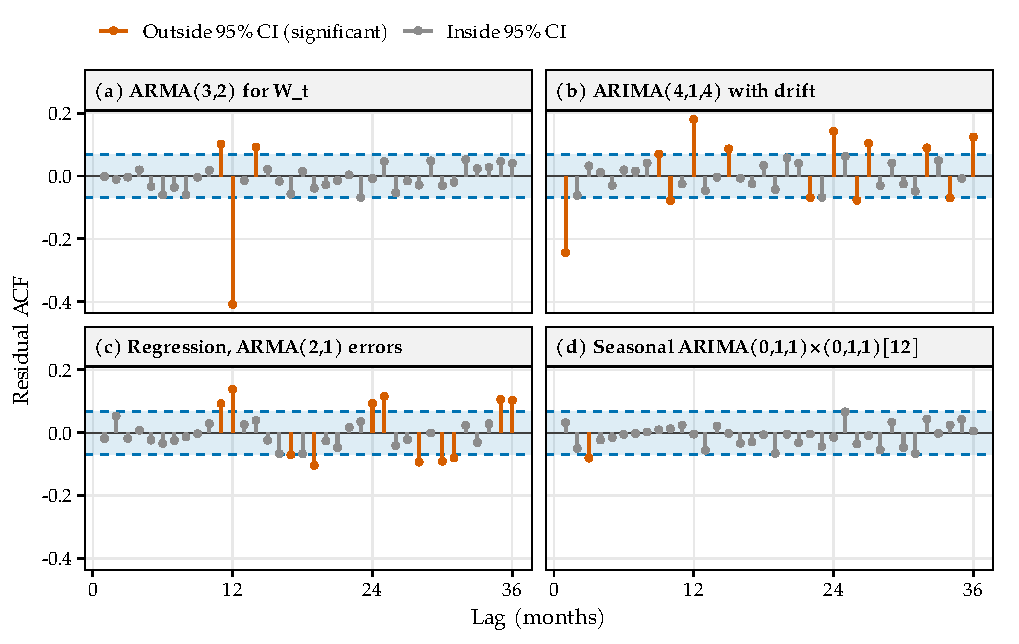
\includegraphics[width=0.82\textwidth]{fig14_residual_acf_by_model_family.pdf}
\end{center}
\note{Backup, use if asked why the other model families were rejected: the residual ACF of the best model in each family. Only the seasonal ARIMA, panel d, has no significant spikes at the seasonal lags 12, 24 and 36.}
\end{frame}

\begin{frame}{Backup: 36-month hold-out forecasts}
\begin{center}
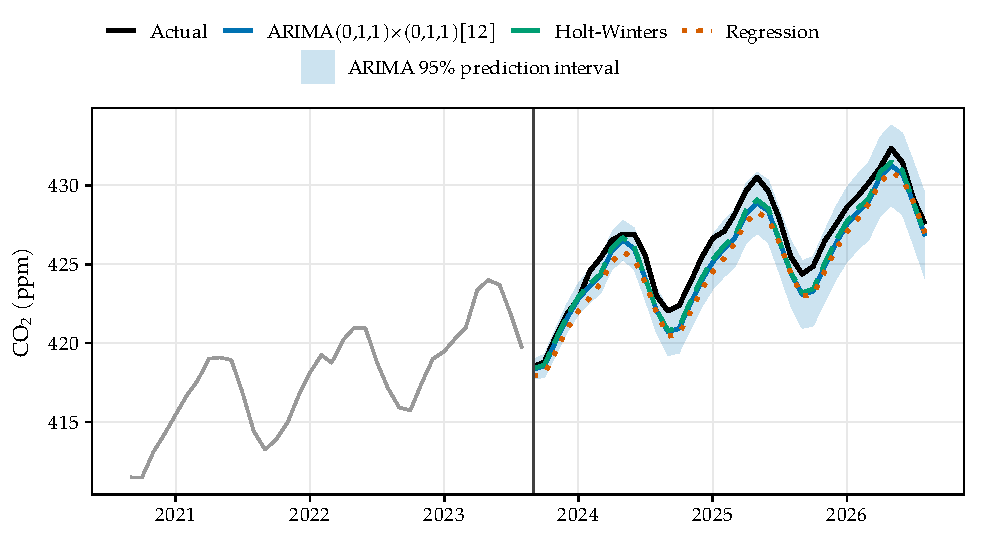
\includegraphics[width=0.86\textwidth]{fig12_holdout_forecast_comparison.pdf}
\end{center}
\note{Backup, use if asked about the recent forecasts: forecasts made in August 2023 for the following three years. All methods under-predicted 2024, the year of record growth during the 2023--24 El Nino, which no univariate model can anticipate.}
\end{frame}

\begin{frame}{Backup: Ljung--Box $p$-values by lag}
\begin{center}
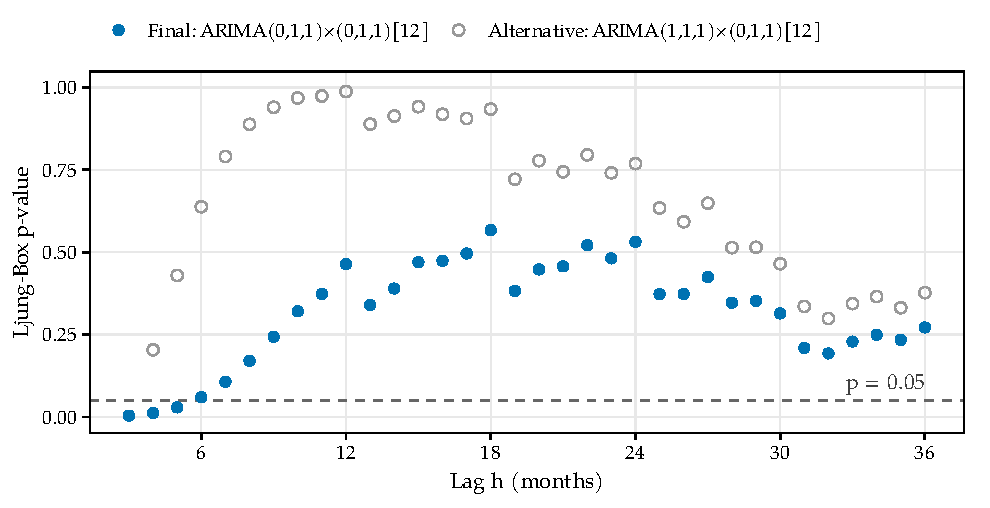
\includegraphics[width=0.86\textwidth]{fig11_ljung_box_pvalues.pdf}
\end{center}
\note{Backup, use if asked about residual independence: Ljung--Box p-values for lags up to 36 for the final and the alternative model. The final model is above 0.05 from lag 6 onwards.}
\end{frame}

\begin{frame}{References}
\scriptsize
\begin{enumerate}[{[}1{]}]\setlength{\itemsep}{1pt}
  \item C.\,D. Keeling (1960). The concentration and isotopic abundances of carbon dioxide in the atmosphere. \emph{Tellus}, 12(2), 200--203. \href{https://doi.org/10.1111/j.2153-3490.1960.tb01300.x}{doi:10.1111/j.2153-3490.1960.tb01300.x}
  \item X.~Lan \& R.\,F. Keeling (2026). Trends in atmospheric carbon dioxide: Mauna Loa monthly mean data. NOAA Global Monitoring Laboratory. \url{https://gml.noaa.gov/ccgg/trends/data.html}
  \item P.\,J. Brockwell \& R.\,A. Davis (2016). \emph{Introduction to Time Series and Forecasting} (3rd ed.). Springer. \href{https://doi.org/10.1007/978-3-319-29854-2}{doi:10.1007/978-3-319-29854-2}
  \item D.\,A. Dickey \& W.\,A. Fuller (1979). Distribution of the estimators for autoregressive time series with a unit root. \emph{JASA}, 74(366), 427--431. \href{https://doi.org/10.1080/01621459.1979.10482531}{doi:10.1080/01621459.1979.10482531}
  \item G.\,E.\,P. Box, G.\,M. Jenkins, G.\,C. Reinsel \& G.\,M. Ljung (2015). \emph{Time Series Analysis: Forecasting and Control} (5th ed.). Wiley. \href{https://search.worldcat.org/title/908107438}{ISBN 978-1-118-67502-1}
  \item G.\,M. Ljung \& G.\,E.\,P. Box (1978). On a measure of lack of fit in time series models. \emph{Biometrika}, 65(2), 297--303. \href{https://doi.org/10.1093/biomet/65.2.297}{doi:10.1093/biomet/65.2.297}
  \item G.~Schwarz (1978). Estimating the dimension of a model. \emph{Annals of Statistics}, 6(2), 461--464. \href{https://doi.org/10.1214/aos/1176344136}{doi:10.1214/aos/1176344136}
  \item P.\,R. Winters (1960). Forecasting sales by exponentially weighted moving averages. \emph{Management Science}, 6(3), 324--342. \href{https://doi.org/10.1287/mnsc.6.3.324}{doi:10.1287/mnsc.6.3.324}
\end{enumerate}
\end{frame}

\end{document}
